\documentclass[12pt]{article}
\usepackage{amsmath,amsthm}
\usepackage{wrapfig}
\usepackage{graphicx}
\usepackage{caption} % Sterge ":" dacă \caption e gol

\renewcommand{\figurename}{Figura}

\newtheorem{definitie}{Definiţia}[subsection]

\begin{document}
\subsection{Legea normală (Gauss-Laplace)}

\begin{definitie}
	Variabila aleatoare $X$ urmează \textbf{legea normală (Gauss-Laplace)} ($X$ are repartiţie normală) cu parametrii $m$ şi $\sigma$ ($m \in R, \sigma > 0$) dacă densitatea de sa de probabilitate (repartiţie) este funcţia
	\begin{equation}
		f(x;m, \sigma) = \frac{1}{\sigma\sqrt{2\pi}} e^{-\frac{(x-m)^2}{2\sigma^2}}, \quad \forall x \in R
	\end{equation}
\end{definitie}

O variabilă aleatoare cu repartiţie normală cu parametrii $m$ şi $\sigma$ se notează cu $N(m, \sigma^2)$.

Funcţia $f$ de mai sus se numeşte \textit{densitatea de repartiţie normală} sau \textit{gaussiană}. Observăm că $f$ este o densitate de probabilitate, deoarece $f(x) > 0, \; \forall x \in R$ şi $\int_{-\infty}^\infty f(x)dx = 1$. Într-adevăr, pentru a verifica ultima relaţie, în integrala de mai sus facem schimbarea de variabilă $\frac{x-m}{\sigma\sqrt{2}} = y$. Rezultă că $dx = \sigma\sqrt{2}dy$. Dacă $x \to -\infty$ atunci $y \to -\infty$, iar dacă $x \to \infty$ atunci $y \to \infty$. Obţinem astfel

\begin{equation*}
\int_{-\infty}^\infty f(x)dx = \frac{1}{\sqrt{\pi}} \int_{-\infty}^\infty e^{-y^2} dy = \frac{2}{\sqrt{\pi}} \int_0^\infty e^{-y^2} dy = 1.
\end{equation*}

\noindent Am folosit mai sus integrala lui Euler-Poisson $\int_0^\infty e^{-y^2}dy = \sqrt{\pi}/2$.


Graficul funcţiei $f$ are formă de clopot (vezi Figura \ref{fig:grafic}). Dreapta de ecuaţie $x=m$ este axă de simetrie pentru acest grafic, iar pentru $x=m$ se obţine valoarea maximă a funcţiei $f$, şi anume $\frac{1}{\sigma \sqrt{2\pi}}$. Punctele $x=m-\sigma$ şi $x=m+\sigma$ sunt puncte de inflexiune.

\begin{wrapfigure}[6cm]{r}{\textwidth}
	\vspace{.2\paperheight}
	\begin{center}
	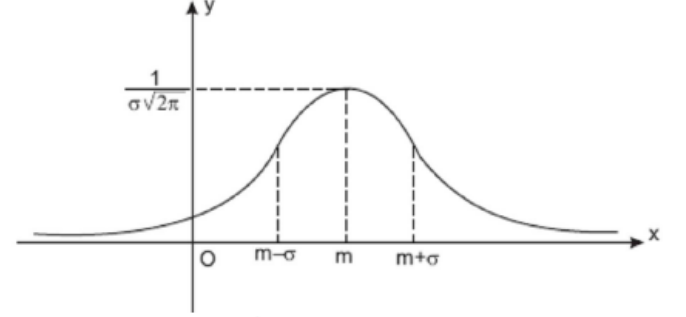
\includegraphics[width=.6\textwidth]{grafic}
	\end{center}
	\caption{\label{fig:grafic}} 
\end{wrapfigure}

\end{document}
